\documentclass[../main/CT4S-EN-RU]{subfiles}

\begin{document}

\section{\caseENGRUS{Groups}{ / }{Группы}}\label{sec:groups}

\begin{blockENG}
Groups are monoids in which every element has an inverse. If we think of these structures in terms of how they act on sets, the difference between groups and monoids is that the action of every group element can be undone. One way of thinking about groups is in terms of symmetries. For example, the rotations and reflections of a square form a group. 
\end{blockENG}

\begin{blockRUS}
Группы — это моноиды, в которых каждый элемент имеет обратный. Если думать об этих структурах в терминах того, как они действуют на множествах, то различие между группами и моноидами в том, что действие каждого элемента группы обратимо. Одним из способов думать о группах являются симметрии. Например, вращения и отражения квадрата образуют группу. 
\end{blockRUS}

\begin{blockENG}
Another way to think of the difference between monoids and groups is in terms of time. Monoids are likely useful in thinking about diffusion, in which time plays a role and things cannot be undone. Groups are more likely useful in thinking about mechanics, where actions are time-reversible. 
\end{blockENG}

\begin{blockRUS}
Есть и другой способ думать о различии между моноидами и группами, основанный на понятии времени. Моноиды хорошо подходят при рассуждениях о диффузии, в которой события нельзя обратить во времени вспять. Группы более подходят для рассуждений о механике, где все события обратимы.
\end{blockRUS}

%%%% Subsection %%%%

\subsection{\caseENGRUS{Definition and examples}{ / }{Определение и примеры}}

\begin{definitionENG}\label{def:group}\index{group}\index{monoid!inverse of an element in}
Let $(M,e,\star)$ be a monoid. An element $m\in M$ is said to {\em have an inverse} if there exists an $m'\in M$ such that $mm'=e$ and $m'm=e.$ A {\em group} is a monoid $(M,e,\star)$ in which every element $m\in M$ has an inverse.
\end{definitionENG}

\begin{definitionRUS}\label{def:group}\index{группа}\index{моноид!обратимый элемент}
Пусть $(M,e,\star)$ — это моноид. Говорят, что элемент $m\in M$ {\em имеет обратный}, если существует такой $m'\in M,$ что $mm'=e$ и $m'm=e.$ {\em Группа} — это моноид $(M,e,\star),$ в котором каждый элемент $m\in M$ имеет обратный.
\end{definitionRUS}

\begin{propositionENG}
Suppose that $\mcM:=(M,e,\star)$ is a monoid and let $m\in M$ be an element. Then $m$ has at most one inverse.%
\footnote{If $\mcM$ is a group then every element $m$ has exactly one inverse.}
\end{propositionENG}

\begin{propositionRUS}
Предположим, что $\mcM:=(M,e,\star)$ — моноид, а $m\in M$ — его элемент. Тогда $m$ имеет не более одного обратного.%
\footnote{Если $\mcM$ — это группа, то каждый элемент $m$ имеет ровно один обратный.}
\end{propositionRUS}

\begin{proofENG}
Suppose that both $m'$ and $m''$ are inverses of $m$; we want to show that $m'=m''.$ This follows by the associative law for monoids:
$$m'=m'(mm'')=(m'm)m''=m''.$$
\end{proofENG}

\begin{proofRUS}
Предположим, что $m'$ и $m''$ являются обратными к $m$; мы хотим показать, что $m'=m''.$ Это следует из свойства ассоциативности моноидов:
$$m'=m'(mm'')=(m'm)m''=m''.$$
\end{proofRUS}

\begin{exampleENG}
The additive monoid $(\NN,0,+)$ is not a group because none of its elements are invertible, except for $0.$ However, the monoid of integers $(\ZZ,0,+)$ is a group. The monoid of clock positions from Example~\ref{ex:cyclic} is also a group. For example the inverse of $Q^5$ is $Q^7$ because $Q^5\star Q^7=e=Q^7\star Q^5.$
\end{exampleENG}

\begin{exampleRUS}
Аддитивный моноид $(\NN,0,+)$ не является группой, поскольку ни один из его элементов не обратим, за исключением $0.$ С другой стороны, аддитивный моноид целых чисел $(\ZZ,0,+)$ — это группа. Моноид позиций часов из Примера~\ref{ex:cyclic} — тоже группа. Например, обратным к $Q^5$ в нем будет $Q^7,$ поскольку $Q^5\star Q^7=e=Q^7\star Q^5.$
\end{exampleRUS}

\begin{exampleENG}
Consider a square centered at the origin in $\RR^2.$ It has rotational and mirror symmetries. There are eight of these, which we denote $$\{e,\rho,\rho^2,\rho^3,\phi,\phi\rho,\phi\rho^2,\phi\rho^3\},$$ where $\rho$ stands for $90^\circ$ counterclockwise rotation and $\phi$ stands for horizontal-flip (across the vertical axis). So relations include $\rho^4=e,$ $\phi^2=e,$ and $\rho^3\phi=\phi\rho.$
\end{exampleENG}

\begin{exampleRUS}
Рассмотрим квадрат в $\RR^2$ с центром в начале координат. Он имеет вращательные и зеркальные симметрии. Всего их восемь, мы обозначим их $$\{e,\rho,\rho^2,\rho^3,\varphi,\varphi\rho,\varphi\rho^2,\varphi\rho^3\},$$ где $\rho$ означает вращение $90^\circ$ против часовой стрелки, а $\varphi$ — горизонтальное отражение (относительно вертикальной оси). Отношения состоят из $\rho^4=e,$ $\varphi^2=e,$ и $\rho^3\varphi=\varphi\rho.$
\end{exampleRUS}

\begin{exampleENG}\label{ex:important groups}
The set of $3\times 3$ matrices can be given the structure of a monoid, where the identity element is the $3\times 3$ identity matrix, the multiplication is matrix multiplication. The subset of invertible matrices forms a group, called {\em the general linear group of dimension 3}\index{a group!$GL_3$} and denoted $GL_3.$ Inside of $GL_3$ is the so-called {\em orthogonal group}, denoted $O_3,$ of matrices $M$ such that $M^\m1=M^\top.$ These matrices correspond to symmetries of the sphere centered at the origin.

Another interesting group is the Euclidean group\index{a group!$E_3$} $E(3)$ which consists of all {\em isometries} of $\RR^3,$ i.e. all functions $\RR^3\to\RR^3$ that preserve distances.  
\end{exampleENG}

\begin{exampleRUS}\label{ex:important groups}
Множеству $3\times 3$ матриц можно придать структуру моноида, где единицей будет единичная матрица $3\times 3,$ а умножением — обычное умножение матриц. Подмножество обратимых матриц образует группу, называемую {\em полной линейной группой порядка 3}\index{группа!$GL_3$} и обозначаемую $GL_3.$ Внутри $GL_3$ имеется так называемая {\em ортогональная группа}, обозначаемая $O_3,$ из таких матриц $M,$ что $M^\m1=M^\top.$ Эти матрицы соответствуют симметриям сферы с центром в начале координат.

Другая интересная группа — Евклидова группа\index{группа!$E_3$} $E(3),$ которая состоит из всех {\em изометрий} $\RR^3,$ т.е. всех функций $\RR^3\to\RR^3,$ сохраняющих растояния.  
\end{exampleRUS}

\begin{applicationENG}\label{app:groups for symmetry}\index{symmetry}
In \href{http://en.wikipedia.org/wiki/Crystallography}{\text crystallography} one is often concerned with the symmetries that arise in the arrangement $A$ of atoms in a molecule. To think about symmetries in terms of groups, we first define an {\em atom-arrangement} to be a finite subset $i\taking A\ss\RR^3.$ A symmetry in this case is an isometry of $\RR^3$ (see Example~\ref{ex:important groups}), say $f\taking\RR^3\to\RR^3$ such that there exists a dotted arrow making the diagram below commute:
$$
\xymatrix{A\ar@{-->}[r]\ar[d]_i&A\ar[d]^i\\\RR^3\ar[r]_f&\RR^3}
$$
That is, it's an isometry of $\RR^3$ such that each atom of $A$ is sent to a position currently occupied by an atom of $A.$ It is not hard to show that the set of such isometries forms a group, called the \href{http://en.wikipedia.org/wiki/Space_group}{\em space group}\index{space group} of the crystal.
\end{applicationENG}

\begin{applicationRUS}\label{app:groups for symmetry}\index{symmetry}
В \href{https://ru.wikipedia.org/wiki/%D0%9A%D1%80%D0%B8%D1%81%D1%82%D0%B0%D0%BB%D0%BB%D0%BE%D0%B3%D1%80%D0%B0%D1%84%D0%B8%D1%8F}{\text кристаллографии} часто интересуются симметриями расположений $A$ атомов в молекуле. Чтобы думать о симметриях в терминах групп, сначала определим {\em расположение атомов} как конечное подмножество $i\taking A\ss\RR^3.$ Симметрия в данном случае — это изометрия $\RR^3$ (см. Пример~\ref{ex:important groups}), скажем такая $f\taking\RR^3\to\RR^3,$ что существует пунктирная стрелка, делающая диаграмму ниже коммутативной:
$$
\xymatrix{A\ar@{-->}[r]\ar[d]_i&A\ar[d]^i\\\RR^3\ar[r]_f&\RR^3}
$$
То есть, это такая изометрия $\RR^3,$ что каждый атом $A$ переходит в положение, занимаемое перед этим (возможно, другим) атомом $A.$ Нетрудно показать, что множество подобных изометрий образует группу, называемую \href{https://ru.wikipedia.org/wiki/%D0%9A%D1%80%D0%B8%D1%81%D1%82%D0%B0%D0%BB%D0%BB%D0%BE%D0%B3%D1%80%D0%B0%D1%84%D0%B8%D1%87%D0%B5%D1%81%D0%BA%D0%B0%D1%8F_%D0%B3%D1%80%D1%83%D0%BF%D0%BF%D0%B0}{\em кристаллографической группой}\index{кристаллографическая группа} данного кристалла.
\end{applicationRUS}

\begin{exerciseENG}\label{exc:permutation}\index{set!permutation of}
Let $S$ be a finite set. A {\em permutation of $S$}\index{permutation} is an isomorphism $f\taking S\To{\iso}S.$ 
\begin{center}
\parbox{2.3in}{
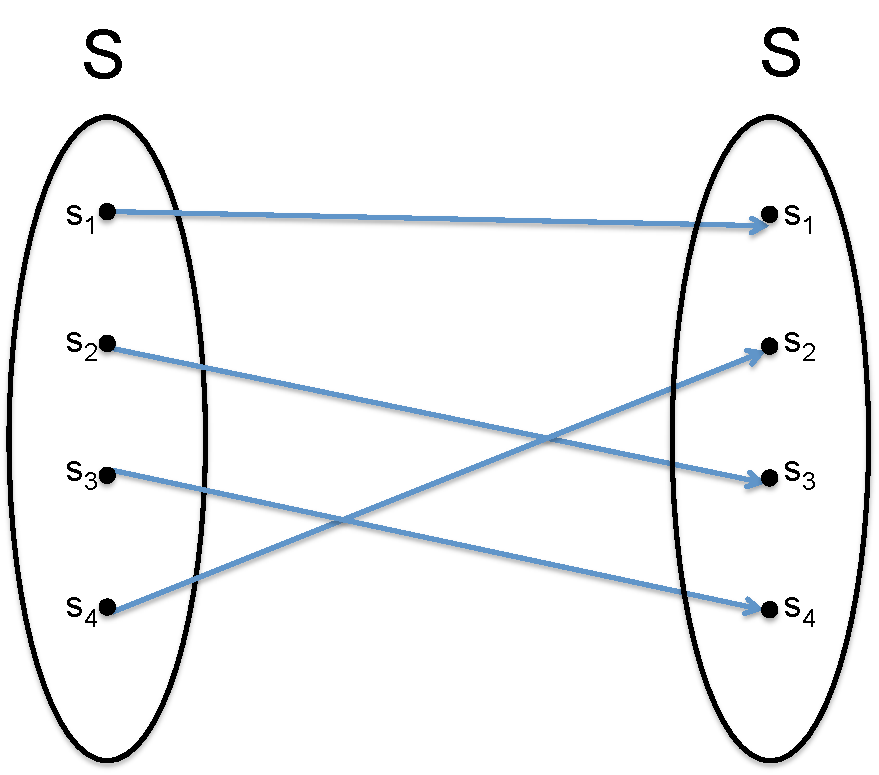
\includegraphics[height=2in]{SetPermutation}}
\end{center}
\sexc Come up with an identity, and a  multiplication formula, such that the set of permutations of $S$ forms a monoid. 
\item Is it a group?
\endsexc
\end{exerciseENG}

\begin{exerciseRUS}\label{exc:permutation}\index{множество!перестановка}
Пусть $S$ — некоторое конечное множество. {\em Перестановка $S$}\index{перестановка} — это изоморфизм $f\taking S\To{\iso}S.$ 
\begin{center}
\parbox{2.3in}{
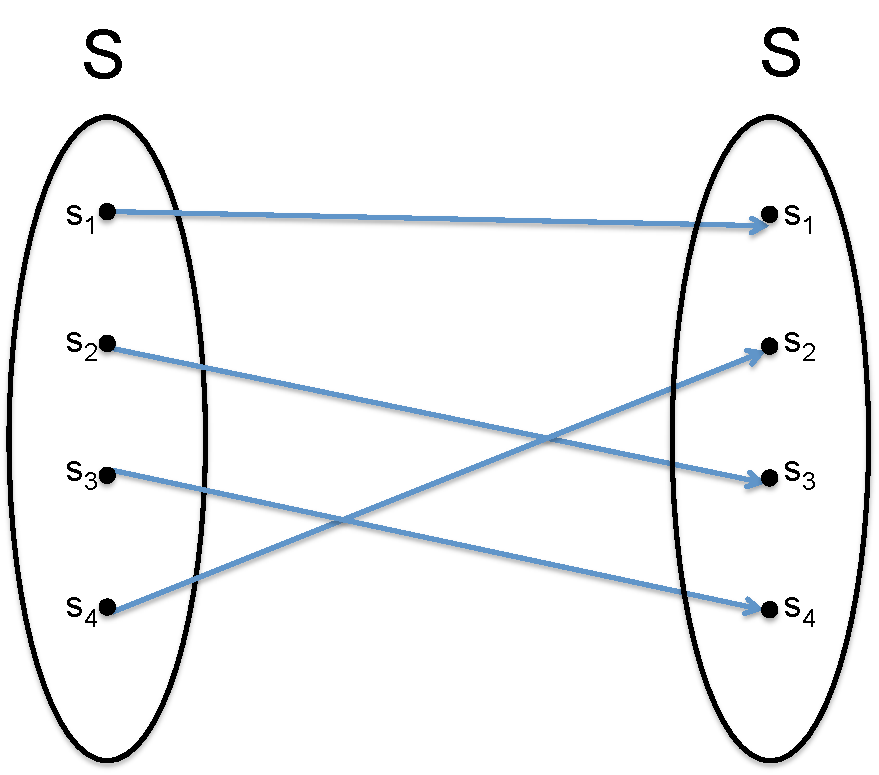
\includegraphics[height=2in]{SetPermutation}}
\end{center}
\sexc Предложите такие данные — единицу и операцию умножения, — что множество перестановок $S$ образует моноид. 
\item Будет ли он группой?
\endsexc
\end{exerciseRUS}

\begin{exerciseENG}
In Exercise~\ref{exc:classify cyclic} you classified the cyclic monoids. Which of them are groups? 
\end{exerciseENG}

\begin{exerciseRUS}
В Упражнении~\ref{exc:classify cyclic} мы классифицировали циклические моноиды. Какие из них оказываются группами? 
\end{exerciseRUS}

\begin{definitionENG}[Group action]\label{def:group action}\index{group!action}\index{action!of a group}
Let $(G,e,\star)$ be a group and $S$ a set. An {\em action} of $G$ on $S$ is a function $\acts\taking G\times S\to S$ such that for all $s\in S$ and $g,g'\in G,$ we have
\begin{itemize}
\item $e\acts s=s$ and
\item $g\acts(g'\acts s)=(g\star g')\acts s.$
\end{itemize}
In other words, considering $G$ as a monoid, it is an action in the sense of Definition~\ref{def:monoid action}.
\end{definitionENG}

\begin{definitionRUS}[Group action]\label{def:group action}\index{group!action}\index{action!of a group}
Пусть $(G,e,\star)$ — некоторая группа, а $S$ — произвольное множество. {\em Действие} $G$ на $S$ — это такая функция $\acts\taking G\times S\to S,$ что для всех $s\in S$ и $g,g'\in G,$ выполняется
\begin{itemize}
\item $e\acts s=s,$
\item $g\acts(g'\acts s)=(g\star g')\acts s.$
\end{itemize}
Другими словами, если считать $G$ моноидом, это будет его действие в смысле Определения~\ref{def:monoid action}.
\end{definitionRUS}

\begin{exampleENG}\label{ex:U(1)}\index{a group!$U(1)$}
When a group acts on a set, it has the character of \href{http://en.wikipedia.org/wiki/Symmetry}{\text symmetry}. For example, consider the group whose elements are angles $\theta.$ This group may be denoted $U(1)$ and is often formalized as the unit circle in $\CC$ of complex numbers $z=a+bi$ such that $|z|=a^2+b^2=1.$ The set of such points is given the structure of a group $(U(1),e,\star)$ by defining the identity element to be $e:=1+0i$ and the group law to be complex multiplication. But for those unfamiliar with complex numbers, this is simply angle addition where we understand that $360^\circ=0^\circ.$ If $\theta_1=190^\circ$ and $\theta_2=278^\circ,$ then $\theta_1\star\theta_2=468^\circ=108^\circ.$ In the language of complex numbers, $z=e^{i\theta}.$

The group $U(1)$ acts on any set that we can picture as having rotational symmetry about a fixed axis, such as the earth around the north-south axis. We will define $S=\{(x,y,z)\in\RR^3\|x^2+y^2+z^2=1\},$ the unit sphere, and understand the rotational action of $U(1)$ on $S.$\index{orbit!rotating earth}

We first show that $U(1)$ acts on $\RR^3$ by $\theta\acts(x,y,z)=(x\cos\theta+y\sin\theta, -x\sin\theta+y\cos\theta,z),$ or with matrix notation as 
$$\theta\acts(x,y,z)
:=(x,y,z)\left(\begin{array}{ccc}
\cos(\theta)&-\sin(\theta)&0\\
\sin(\theta)&\cos(\theta)&0\\
0&0&1\end{array}\right)
$$
\href{http://en.wikipedia.org/wiki/List_of_trigonometric_identities#Matrix_form}{\text Trigonometric identities} ensure that this is indeed an action.

In terms of action tables, we would need infinitely many columns to express this action. Here is a sample
$$
\begin{tabular}{| l || l | l | l |}
\bhline
\multicolumn{4}{|c|}{Action of $U(1)$ on $\RR^3$}\\\bhline
{$\RR^3$}&{$\theta=45^\circ$}&{$\theta=90^\circ$}&{$\theta=100^\circ$}\\\bbhline
(0,0,0)&(0,0,0)&(0,0,0)&(0,0,0)\\\hline
(1,0,0)&(.71,.71,0)&(0,1,0)&(-.17,.98,0)\\\hline
(0,1,-4.2)&(-.71,.71,-4.2)&(-1,0,-4.2)&(-.98,-.17,-4.2)\\\hline
(3,4,2)&(4.95,.71,2)&(-4,3,2)&(3.42,-3.65,2)\\\hline
$\vdots$&$\vdots$&$\vdots$&$\vdots$\\\bhline
\end{tabular}
$$

Finally, we are looking to see that the action preserves length so that if $(x,y,z)\in S$ then $\theta\acts(x,y,z)\in S$; this way we will have confirmed that $U(1)$ indeed acts on $S.$ The calculation begins by assuming $x^2+y^2+z^2=1$ and checks 
$$
(x\cos\theta+y\sin\theta)^2+(-x\sin\theta+y\cos\theta)^2+z^2=x^2+y^2+z^2=1.
$$
\end{exampleENG}

\begin{exampleRUS}\label{ex:U(1)}\index{a group!$U(1)$}
Когда группа действует на множестве, она имеет характер \href{https://ru.wikipedia.org/wiki/%D0%A1%D0%B8%D0%BC%D0%BC%D0%B5%D1%82%D1%80%D0%B8%D1%8F}{\text симметрии}. Например, рассморим группу, элементами которой являются углы $\theta.$ Эту группу обозначают $U(1)$ и зачастую формализуют как единичную окружность на плоскости $\CC,$ состоящую из таких комплексных чисел $z=a+bi,$ что $|z|=a^2+b^2=1.$ Множество этих точек получает структуру группы $(U(1),e,\star),$ если задать в качестве единицы число $e:=1+0i,$ а в качестве умножения — обычное умножение комплекных чисел. Тем, для кого комплексные числа не столь привычны, сообщаем, что это просто сложение углов, где мы учитываем, что $360^\circ=0^\circ.$ Если $\theta_1=190^\circ$ и $\theta_2=278^\circ,$ то $\theta_1\star\theta_2=468^\circ=108^\circ.$ На языке комплексных чисел, $z=e^{i\theta}.$

Группа $U(1)$ действует на любое множество, в котором обнаруживается вращательная симметрия вокруг фиксированной оси, подобная вращению Земли вокруг оси между Южным и Северным полюсами. Мы обозначим $S=\{(x,y,z)\in\RR^3\|x^2+y^2+z^2=1\}$ единичную сферу, и изучим действие вращением группы $U(1)$ на множество $S.$\index{орбита!вращения Земли}

Сначала покажем, что $U(1)$ действует на $\RR^3$ так: $\theta\acts(x,y,z)=(x\cos\theta+y\sin\theta, -x\sin\theta+y\cos\theta,z)$ или в матричной записи
$$\theta\acts(x,y,z)
:=(x,y,z)\left(\begin{array}{ccc}
\cos(\theta)&-\sin(\theta)&0\\
\sin(\theta)&\cos(\theta)&0\\
0&0&1\end{array}\right)
$$
\href{https://ru.wikipedia.org/wiki/%D0%A2%D1%80%D0%B8%D0%B3%D0%BE%D0%BD%D0%BE%D0%BC%D0%B5%D1%82%D1%80%D0%B8%D1%87%D0%B5%D1%81%D0%BA%D0%B8%D0%B5_%D1%82%D0%BE%D0%B6%D0%B4%D0%B5%D1%81%D1%82%D0%B2%D0%B0}{\text Тригонометрические тождества} гарантируют нам, что это действительно действие.

В терминах таблиц действия для выражения этого действия нам бы потребовалось бесконечно много столбцов. Вот пример:
$$
\begin{tabular}{| l || l | l | l |}
\bhline
\multicolumn{4}{|c|}{Action of $U(1)$ on $\RR^3$}\\\bhline
{$\RR^3$}&{$\theta=45^\circ$}&{$\theta=90^\circ$}&{$\theta=100^\circ$}\\\bbhline
(0,0,0)&(0,0,0)&(0,0,0)&(0,0,0)\\\hline
(1,0,0)&(.71,.71,0)&(0,1,0)&(-.17,.98,0)\\\hline
(0,1,-4.2)&(-.71,.71,-4.2)&(-1,0,-4.2)&(-.98,-.17,-4.2)\\\hline
(3,4,2)&(4.95,.71,2)&(-4,3,2)&(3.42,-3.65,2)\\\hline
$\vdots$&$\vdots$&$\vdots$&$\vdots$\\\bhline
\end{tabular}
$$

Наконец, мы собираемся проверить, что данное действие сохраняет расстояния так, что если $(x,y,z)\in S,$ то $\theta\acts(x,y,z)\in S$; таким образом мы убедимся в том, что $U(1)$ действительно действует на $S.$ Начнем вычисления с известного равенства $x^2+y^2+z^2=1$ и получим, что 
$$
(x\cos\theta+y\sin\theta)^2+(-x\sin\theta+y\cos\theta)^2+z^2=x^2+y^2+z^2=1.
$$
\end{exampleRUS}

\begin{exerciseENG}\label{exc:permutation group}
Let $X$ be a set and consider the group of permutations of $X$ (see Exercise~\ref{exc:permutation}), which we will denote $\Sigma_X$\index{a group!$\Sigma_X$}. Find a canonical action of $\Sigma_X$ on $X.$
\end{exerciseENG}

\begin{exerciseRUS}\label{exc:permutation group}
Пусть $X$ — некоторое множество; рассмотрим группу перестановок $X$ (см. Пример~\ref{exc:permutation}), которую мы обозначим $\Sigma_X$\index{группа!$\Sigma_X$}. Найдите каноническое действие $\Sigma_X$ на $X.$
\end{exerciseRUS}

\begin{definitionENG}
Let $G$ be a group acting on a set $X.$ For any point $x\in X,$ the {\em orbit of $x$},\index{orbit}\index{action!orbit of} denoted $Gx,$ is the set 
$$Gx:=\{x'\in X\|\exists g\in G \tn{ such that }gx=x'\}.$$
\end{definitionENG}

\begin{definitionRUS}
Пусть $G$ — некоторая группа, действующая на множестве $X.$ Для любой точки $x\in X$ {\em орбита $x$},\index{орбита}\index{действие!орбита} обозначаемая $Gx,$ — это множество
$$Gx:=\{x'\in X\|\exists g\in G \tn{ такой, что }gx=x'\}.$$
\end{definitionRUS}

\begin{applicationENG}
Let $S$ be the surface of the earth, understood as a sphere, and let $G=U(1)$ be the group of angles acting on $S$ as in Example~\ref{ex:U(1)}. The orbit of any point $p=(x,y,z)\in S$ is the set of points on the same latitude line as $p.$

One may also consider a small band around the earth, i.e. the set $A=\{(x,y,z)\|1.0\leq x^2+y^2+z^2\leq 1.05\}.$ The action of $U(1)\acts S$ extends to an action $U(1)\acts A.$ The orbits are latitude-lines-at-altitude. A simplifying assumption in \href{http://en.wikipedia.org/wiki/Climatology}{\text climatology} may be given by assuming that $U(1)$ acts on all currents in the atmosphere in an appropriate sense. That way, instead of considering movement within the whole space $A,$ we only allow movement that behaves the same way throughout each orbit of the group action.
\end{applicationENG}

\begin{applicationRUS}
Пусть $S$ — это поверхность Земли, которую мы считаем сферой, и пусть $G=U(1)$ — группа углов, действующая на $S$ как в Примере~\ref{ex:U(1)}. Орбита любой точки $p=(x,y,z)\in S$ — это множество точек с той же самой широтой, что у $p.$

Можно также рассмотреть небольшой слой вокруг Земли, т.е. множество $A=\{(x,y,z)\|1.0\leq x^2+y^2+z^2\leq 1.05\}.$ Действие $U(1)\acts S$ расширяется до действия $U(1)\acts A.$ Орбитами будут «линии широты на определенной высоте». Одним из упрощенных положений \href{https://ru.wikipedia.org/wiki/%D0%9A%D0%BB%D0%B8%D0%BC%D0%B0%D1%82%D0%BE%D0%BB%D0%BE%D0%B3%D0%B8%D1%8F}{\text климатологии} является предположение о том, что $U(1)$ в определенном смысле действует на все атмосферные потоки. Тогда вместо того, чтобы рассматривать движения во всем пространстве $A,$ мы разрешаем только такие движения, которые ведут себя одинаковым образом на каждой орбите данного действия группы.
\end{applicationRUS}

\begin{exerciseENG}~
\sexc Consider the $U(1)$ action on $\RR^3$ given in Example~\ref{ex:U(1)}. Describe the set of orbits of this action.
\item What are the orbits of the action of the permutation group $\Sigma_{\{1,2,3\}}$ on the set $\{1,2,3\}?$ (See Exercise~\ref{exc:permutation group}.)
\endsexc
\end{exerciseENG}

\begin{exerciseRUS}~
\sexc Рассмотрим действие $U(1)$ на $\RR^3,$ описанное в Примере~\ref{ex:U(1)}. Опишите множество орбит этого действия.
\item Каковы орбиты действия группы перестановок $\Sigma_{\{1,2,3\}}$ на множестве $\{1,2,3\}?$ (См. Упражнение~\ref{exc:permutation group}.)
\endsexc
\end{exerciseRUS}

\begin{exerciseENG}
Let $G$ be a group and $X$ a set on which $G$ acts by $\acts\taking G\times X\to X.$ Is “being in the same orbit” an equivalence relation on $X?$ 
\end{exerciseENG}

\begin{exerciseRUS}
Пусть $G$ — некоторая группа, а $X$ — множество, на котором $G$ действует при помощи $\acts\taking G\times X\to X.$ Является ли «расположены на одной орбите» отношением эквивалентности на $X?$ 
\end{exerciseRUS}

\begin{definitionENG}\label{def:group homomorphism}\index{group!homomorphism of}
Let $G$ and $G'$ be groups. A {\em group homomorphism} $f\taking G\to G'$ is defined to be a monoid homomorphism $G\to G',$ where $G$ and $G'$ are being regarded as monoids in accordance with Definition~\ref{def:group}.
\end{definitionENG}

\begin{definitionRUS}\label{def:group homomorphism}\index{group!homomorphism of}
Пусть $G$ и $G'$ — некоторые группы. {\em Гомоморфизм групп} $f\taking G\to G'$ определяется как гомоморфизм моноидов $G\to G',$ где $G$ и $G'$ рассматриваются как моноиды в соответствии с Определением~\ref{def:group}.
\end{definitionRUS}

\end{document}
